\documentclass[10pt,letterpaper]{article}\usepackage[]{graphicx}\usepackage[]{color}
%% maxwidth is the original width if it is less than linewidth
%% otherwise use linewidth (to make sure the graphics do not exceed the margin)
\makeatletter
\def\maxwidth{ %
  \ifdim\Gin@nat@width>\linewidth
    \linewidth
  \else
    \Gin@nat@width
  \fi
}
\makeatother

\definecolor{fgcolor}{rgb}{0.345, 0.345, 0.345}
\newcommand{\hlnum}[1]{\textcolor[rgb]{0.686,0.059,0.569}{#1}}%
\newcommand{\hlstr}[1]{\textcolor[rgb]{0.192,0.494,0.8}{#1}}%
\newcommand{\hlcom}[1]{\textcolor[rgb]{0.678,0.584,0.686}{\textit{#1}}}%
\newcommand{\hlopt}[1]{\textcolor[rgb]{0,0,0}{#1}}%
\newcommand{\hlstd}[1]{\textcolor[rgb]{0.345,0.345,0.345}{#1}}%
\newcommand{\hlkwa}[1]{\textcolor[rgb]{0.161,0.373,0.58}{\textbf{#1}}}%
\newcommand{\hlkwb}[1]{\textcolor[rgb]{0.69,0.353,0.396}{#1}}%
\newcommand{\hlkwc}[1]{\textcolor[rgb]{0.333,0.667,0.333}{#1}}%
\newcommand{\hlkwd}[1]{\textcolor[rgb]{0.737,0.353,0.396}{\textbf{#1}}}%
\let\hlipl\hlkwb

\usepackage{framed}
\makeatletter
\newenvironment{kframe}{%
 \def\at@end@of@kframe{}%
 \ifinner\ifhmode%
  \def\at@end@of@kframe{\end{minipage}}%
  \begin{minipage}{\columnwidth}%
 \fi\fi%
 \def\FrameCommand##1{\hskip\@totalleftmargin \hskip-\fboxsep
 \colorbox{shadecolor}{##1}\hskip-\fboxsep
     % There is no \\@totalrightmargin, so:
     \hskip-\linewidth \hskip-\@totalleftmargin \hskip\columnwidth}%
 \MakeFramed {\advance\hsize-\width
   \@totalleftmargin\z@ \linewidth\hsize
   \@setminipage}}%
 {\par\unskip\endMakeFramed%
 \at@end@of@kframe}
\makeatother

\definecolor{shadecolor}{rgb}{.97, .97, .97}
\definecolor{messagecolor}{rgb}{0, 0, 0}
\definecolor{warningcolor}{rgb}{1, 0, 1}
\definecolor{errorcolor}{rgb}{1, 0, 0}
\newenvironment{knitrout}{}{} % an empty environment to be redefined in TeX

\usepackage{alltt}
\usepackage[top=0.85in,left=1.75in,footskip=0.75in]{geometry}

% amsmath and amssymb packages, useful for mathematical formulas and symbols
\usepackage{amsmath,amssymb}

% Use adjustwidth environment to exceed column width (see example table in text)
\usepackage{changepage}

% Use Unicode characters when possible
\usepackage[utf8x]{inputenc}

% textcomp package and marvosym package for additional characters
\usepackage{textcomp,marvosym}

% cite package, to clean up citations in the main text. Do not remove.
\usepackage{cite}

% Use nameref to cite supporting information files (see Supporting Information section for more info)
\usepackage{nameref,hyperref}

% line numbers
\usepackage[right]{lineno}

% ligatures disabled
\usepackage{microtype}
\DisableLigatures[f]{encoding = *, family = * }

% color can be used to apply background shading to table cells only
\usepackage[table]{xcolor}

% array package and thick rules for tables
\usepackage{array}

% bold math symbols package
\usepackage{bm}

% nice figures and captions
\usepackage{graphicx}

% diagrams or complicated equations
\usepackage{tikz}

% vertical and horizontal dashed lines
\usepackage{arydshln}

%\usepackage{floatflt}
%\usepackage{nonfloat}
\usepackage{float}
\usepackage{wrapfig}

%\renewcommand{\arraystretch}{1.2}
%\setlength{\tabcolsep}{12pt}

% create "+" rule type for thick vertical lines
\newcolumntype{+}{!{\vrule width 2pt}}

% create \thickcline for thick horizontal lines of variable length
\newlength\savedwidth
\newcommand\thickcline[1]{%
  \noalign{\global\savedwidth\arrayrulewidth\global\arrayrulewidth 2pt}%
  \cline{#1}%
  \noalign{\vskip\arrayrulewidth}%
  \noalign{\global\arrayrulewidth\savedwidth}%
}

% \thickhline command for thick horizontal lines that span the table
\newcommand\thickhline{\noalign{\global\savedwidth\arrayrulewidth\global\arrayrulewidth 2pt}%
\hline
\noalign{\global\arrayrulewidth\savedwidth}}


% Remove comment for double spacing
%\usepackage{setspace} 
%\doublespacing

% Text layout
% \raggedright
\setlength{\parindent}{0.5cm}
\textwidth 5.25in 
\textheight 8.75in

% Bold the 'Figure #' in the caption and separate it from the title/caption with a period
% Captions will be left justified
\usepackage[aboveskip=1pt,labelfont=bf,labelsep=period,justification=raggedright,singlelinecheck=off]{caption}
\renewcommand{\figurename}{Fig}

% Use the PLoS provided BiBTeX style
%\bibliographystyle{plos2015}


% Remove brackets from numbering in List of References
\makeatletter
\renewcommand{\@biblabel}[1]{\quad#1.}
\makeatother

% define theorem and definition environments commands
\newtheorem{theorem}{Theorem}[section]
\newtheorem{definition}{Definition}[section]

% Header and Footer with logo
\usepackage{lastpage,fancyhdr,graphicx}
\usepackage{epstopdf}
%\pagestyle{myheadings}
\pagestyle{fancy}
\fancyhf{}
%\setlength{\headheight}{27.023pt}
%\lhead{\includegraphics[width=2.0in]{PLOS-submission.eps}}
\rfoot{\thepage/\pageref{LastPage}}
\renewcommand{\headrulewidth}{0pt}
\renewcommand{\footrule}{\hrule height 2pt \vspace{2mm}}
\fancyheadoffset[L]{2.25in}
% \fancyfootoffset[L]{1.25in}
\lfoot{\today}


\restylefloat{figure}


%% Include all macros below

\newcommand{\lorem}{{\bf LOREM}}
\newcommand{\ipsum}{{\bf IPSUM}}

\def\lf{\left\lfloor}   
\def\rf{\right\rfloor}

\def\ri{R_i}
\def\rj{R_j}
\def\kmi{k_{M_i}}
\def\khi{k_{H_i}}
\def\hji{H_{j_i}}
\def\ma{\overline{M}_a}
\def\ha{\overline{H}_a}
\def\mnu{M_\nu}
\def\hnu{H_\nu}
\def\myd{\text{diff}}
\def\ka{\bar{k}_\alpha}
\def\mji{M_{j_i}}

%% END MACROS SECTION
\IfFileExists{upquote.sty}{\usepackage{upquote}}{}
\begin{document}
\vspace*{0.2in}

% Title must be 250 characters or less.
% \begin{flushleft}
{\Large
\textbf\newline{Blessings of Dimensionality: Finding the optimal k for nearest-neighbor projected-distance feature selection (for detecting interaction and main effects in high dimensional data)} % Please use "sentence case" for title and headings (capitalize only the first word in a title (or heading), the first word in a subtitle (or subheading), and any proper nouns).
}
%\newline
% Insert author names, affiliations and corresponding author email (do not include titles, positions, or degrees).
\begin{center}
  \begin{tabular}{l}
  Bryan A. Dawkins$^{\text{1}}$, Trang T. Le$^{\text{2}}$ and Brett A. McKinney$^{\text{1,3,}*}$ \\
  $^{\text{1}}$Department of Mathematics, University of Tulsa, Tulsa, OK 74104, USA \\
  $^{\text{2}}$Department of Biostatistics, Epidemiology and Informatics, University of \\
  \hphantom{2}Pennsylvania, Philadelphia, PA 19104 \\
  $^{\text{3}}$Tandy School of Computer Science, University of Tulsa, Tulsa, OK 74104, USA.
  \end{tabular}
\end{center}


% \end{flushleft}
% Please keep the abstract below 300 words
\section*{Abstract}
It is commonly known that high-throughput data has many inherent statistical challenges, such as multiple testing, sparsity and over fitting. Collectively, these challenges are known as the Curse of Dimensionality. Here we highlight an important Blessing of Dimensionality: the ability to identify interactions with neighborhoods of instances. We review the nearest-neighbor concept for finding interactions among attributes. We present a novel simulation method for generating interactions from random networks with fine-tuned control over interaction effect size. Using our new simulation strategy, we determine optimal fixed-$k$ for neighborhood computation in nearest-neighbor distance-based feature selection for different combinations of data dimensions $m$ (number of instances) and $p$ (number of attributes), different ratios of main/interaction effect among functional attributes, and different combinations of main and interaction effect sizes. We discuss ways to maximize the blessings and minimize the curses of dimensionality to reliably identify interactions. Our results will show how optimal fixed-$k$ changes under a variety of conditions that we see in real data, which will serve as a guide for other researchers using nearest-neighbor distance-based feature selection. 

\section*{Author summary}

\linenumbers

\section*{Introduction}

Relief-based methods identify interacting attributes as important by using nearest-neighbor information in higher dimensions (the ``blessings of dimensionality''). Myopic methods that do not account for information from higher dimensions such as univariate tests are susceptible to false negatives when there are interactions. For example, in the plot of variable A versus C in a three-variable simulation (Fig.~\ref{fig:ABC}-I), variable A appears to show no difference between cases and controls (the marginal group means are the same). However, A is actually simulated to have a strong differential correlation with B, conditioned on the outcome variable (Fig.~\ref{fig:ABC}-II). Current Relief-based methods determine the importance of an attribute by computing the average difference of attribute $A$ value between a target instance (X) and its nearest instance from the opposite class (Miss), $d_{\text{X,M}}(A)$, subtracted from the similarly projected difference of target X and its nearest instance from the same class (Hit), $d_{\text{X,H}}(A)$. A positive value from this calculation, i.e., $d_{\text{X,M}}(A)-d_{\text{X,H}}(A) > 0$, suggests that attribute A is useful for discriminating between cases and controls.  

\begin{figure}[H]
	\centering
	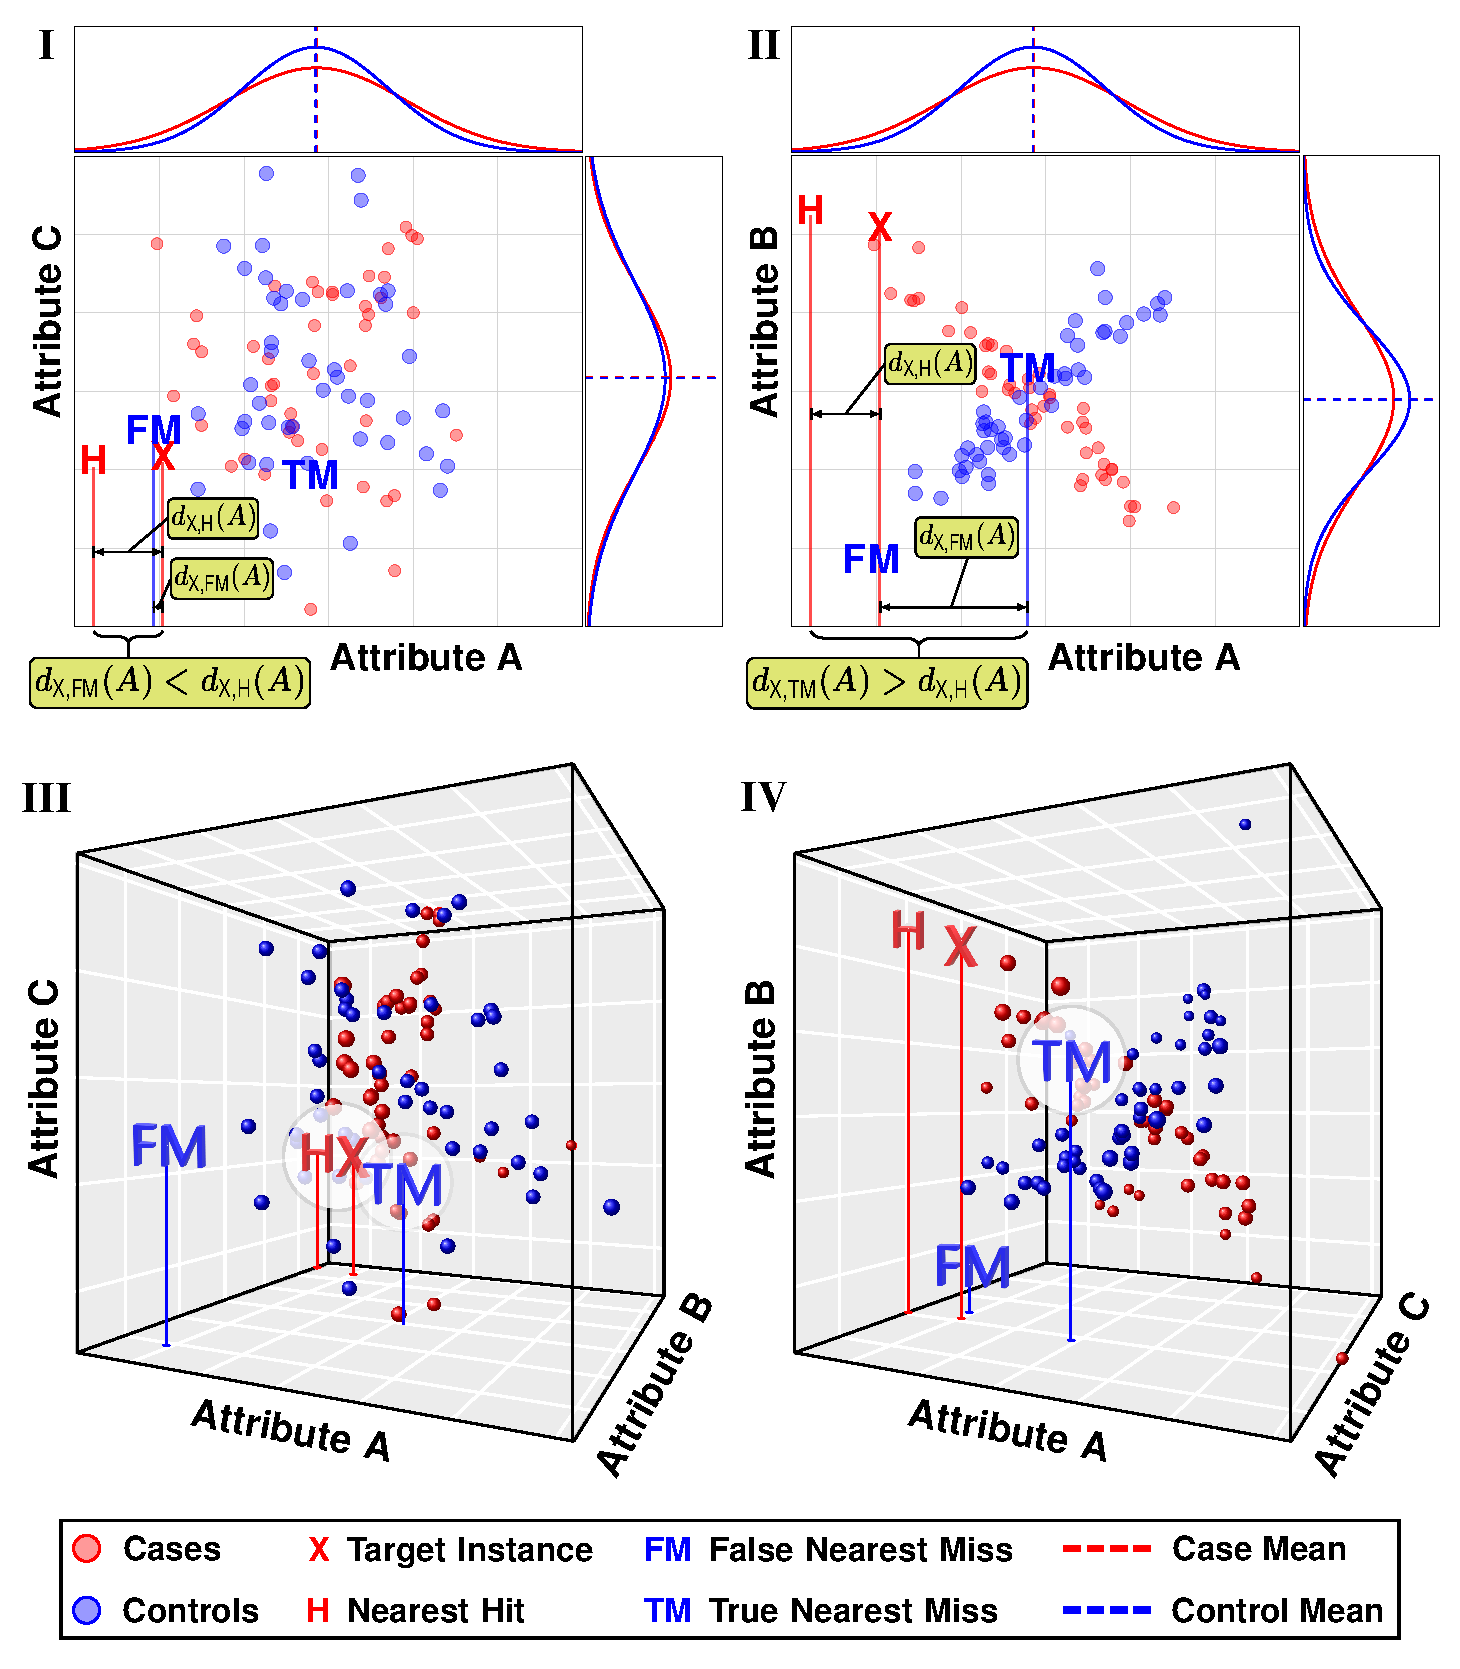
\includegraphics[width=\textwidth]{2by2_arrangementABC.pdf}
	\caption{{\bf Imposters vs true neighbors in the presence of interactions with three variables}. Attributes A, B, and C have no main effect. (\textbf{\fontfamily{ptm}\selectfont I}) Scatter plot of simulated irrelevant Attribute C with a functional Attribute A. (\textbf{\fontfamily{ptm}\selectfont II}) Scatter plot of Attributes A and B, which interact through differential correlation. Computing nearest neighbors with irrelevant attributes (\textbf{\fontfamily{ptm}\selectfont I}) or lower dimensions leads to imposter nearest neighbors and degrades the ability of Relief-based methods to identify interaction effects. Computing distances in only these two dimensions leads to an imposter false miss (FM) for the nearest neighbor from the opposite outcome class for target instance X. This imposter leads to Attribute A predicting closer projected distances for misses than hits (H), which incorrectly indicates that A is a poor discriminator (yellow boxes in \textbf{\fontfamily{ptm}\selectfont I}). (\textbf{\fontfamily{ptm}\selectfont III-IV}) Computing nearest neighbors in higher dimensions or with the correct interaction partner leads to imposter nearest neighbor (FM) being replaced by the true nearest miss neighbor (TM) for target instance X, which correctly leads to Attribute A predicting closer projected distances for hits (H) than misses, which is an indication that Attribute A is a good discriminator (yellow boxes \textbf{\fontfamily{ptm}\selectfont II}).}\label{fig:ABC}
\end{figure}
%\begin{figure}[h!]
%%\begin{center}
%\begin{minipage}[c]{0.4\textheight}
%\centering
%		\framebox{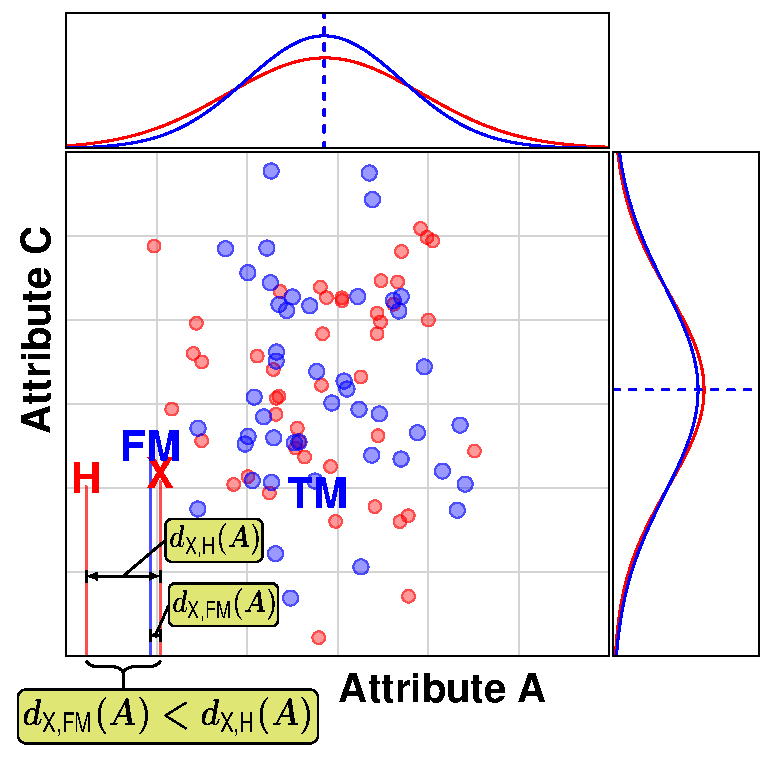
\includegraphics[width=0.8\textwidth]{glmSTIR_figure_2D_final_CvsA.pdf}}
%\end{minipage} \hspace{-0.4cm}
%\begin{minipage}[c]{0.5\textwidth}
%\centering
%\caption{{\bf Imposters vs true neighbors in the presence of interactions with three variables}. Scatter plot of simulated irrelevant Attribute C with a functional Attribute A {\bf(a)}. None of the attributes has a main effect, but Attribute B and C interact through differential correlation {\bf(b)}. Computing nearest neighbors with irrelevant attributes {\bf(a)} or lower dimensions leads to imposter nearest neighbors and degrades the ability of Relief-based methods to identify interaction effects. Computing distances in only these two dimensions leads to an imposter false miss (FM) for the nearest neighbor from the opposite outcome class for target instance X. This imposter leads to attribute A predicting closer projected distances for misses than hits (H), which incorrectly indicates that A is a poor discriminator (yellow boxes in {\bf a}). Computing nearest neighbors in higher dimensions {\bf(c-d)} or with the correct interaction partner leads to imposter nearest neighbor (FM) being replaced by the true nearest miss neighbor (TM) for target instance X, which correctly leads to attribute A predicting closer projected distances for hits (H) than misses, which is an indication that attribute A is a good discriminator (yellow boxes {\bf(b)}).}\label{fig:2dAvC}
%\end{minipage}
%%\end{center}
%\end{figure}

\newpage

%\begin{figure}[ht!]
%\begin{wrapfigure}{l}{0.6\textwidth}
%    \vspace{-12pt}
%	\centering
%	\framebox{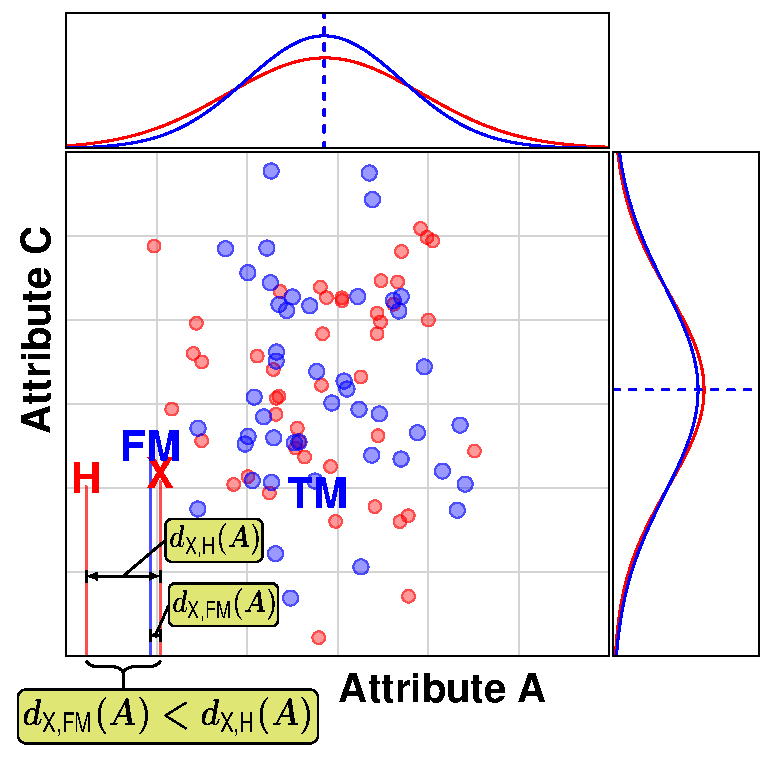
\includegraphics[width=0.55\textwidth]{glmSTIR_figure_2D_final_CvsA.pdf}}
%\end{wrapfigure}
%\noindent\refstepcounter{figure}\textbf{Fig \thefigure \label{fig:2dAvC}.} \textbf{Imposters vs true neighbors in the presence of interactions with three variables}. Scatter plot of simulated irrelevant Attribute C with a functional Attribute A \textbf{(a)}. None of the attributes has a main effect, but Attribute B and C interact through differential correlation \textbf{(b)}. Computing nearest neighbors with irrelevant attributes \textbf{(a)} or lower dimensions leads to imposter nearest neighbors and degrades the ability of Relief-based methods to identify interaction effects. Computing distances in only these two dimensions leads to an imposter false miss (FM) for the nearest neighbor from the opposite outcome class for target instance X. This imposter leads to attribute A predicting closer projected distances for misses than hits (H), which incorrectly indicates that A is a poor discriminator (yellow boxes in \textbf{(a)}). Computing nearest neighbors in higher dimensions \textbf{(c-d)} or with the correct interaction partner leads to imposter nearest neighbor (FM) being replaced by the true nearest miss neighbor (TM) for target instance X, which correctly leads to attribute A predicting closer projected distances for hits (H) than misses, which is an indication that attribute A is a good discriminator (yellow boxes \textbf{(b)}).
%\end{figure}

Relief-based methods use information from all available attributes (omnigenic) to estimate an attribute's importance. However, if relevant higher-dimensional information is not used to establish the neighborhoods of instances, these methods will miss the effect of A because ``imposter'' neighbors will be used in the attribute estimate (False Miss (FM) in Fig.~\ref{fig:ABC}-I, where $d_{\text{X,FM}}(A)<d_{\text{X,H}}(A)$).  If one were to compute nearest neighbors in the A-C plane (ignoring the B dimension), the nearest miss would be an imposter (FM), which leads to a negative contribution to the importance score for A. One might call this C attribute a type-I confounding attribute because it increases the chances of interacting attributes to be false negatives. When nearest neighbors are calculated based on higher dimensions with relevant information (Fig.~\ref{fig:ABC}-III), it is clear that TM is closer to X than FM. The imposter (FM) is replaced by the true nearest miss (TM) and attribute A correctly shows a greater projected difference between misses than hits (Fig.~\ref{fig:ABC}-II $d_{\text{X,TM}}(A)>d_{\text{X,H}}(A)$), which is the signature of an important attribute. Univariate methods still cannot find the importance of A unless the interaction is explicitly modeled, but as long as functional variables A and B are in the space for nearest neighbor calculations (Fig.~\ref{fig:ABC}-III - IV), imposters can be excluded and Relief-based methods will find that A (and B) are important discriminators. 



%\begin{figure}[ht!]
%%\begin{center}
%\begin{minipage}[c]{0.4\textheight}
%\centering 
%		\framebox{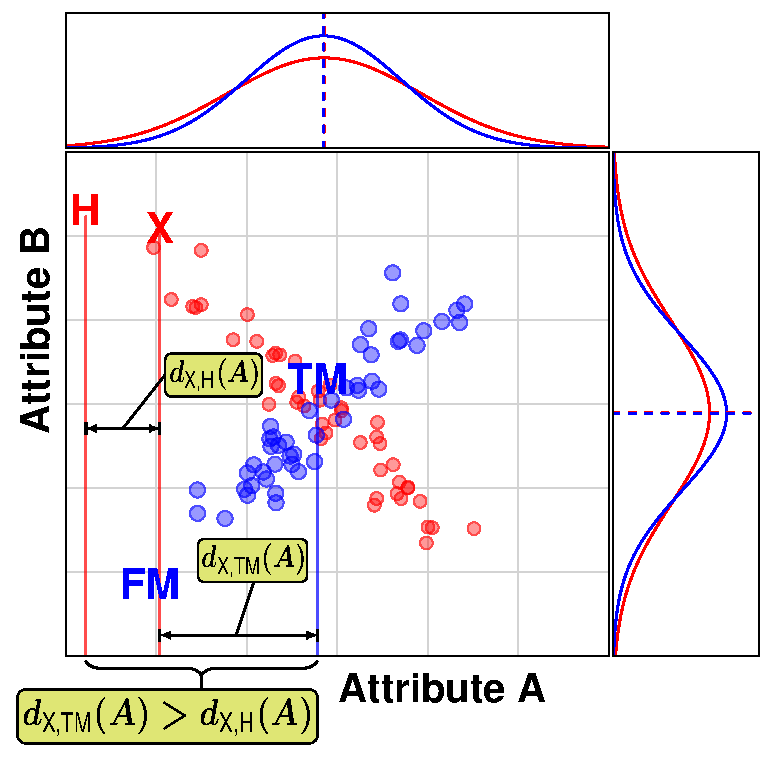
\includegraphics[width=0.8\textwidth]{glmSTIR_figure_2D_final_BvsA.pdf}}
%\end{minipage} \hspace{-0.4cm}
%\begin{minipage}[c]{0.5\textwidth}
%\centering
%\caption{{\bf True neighbors}}\label{fig:2dAvB}
%\end{minipage}
%%\end{center}
%\end{figure}  

%\begin{figure}[ht!]
%%\begin{center}
%\begin{minipage}[c]{0.4\textheight}
%\centering
%		\framebox{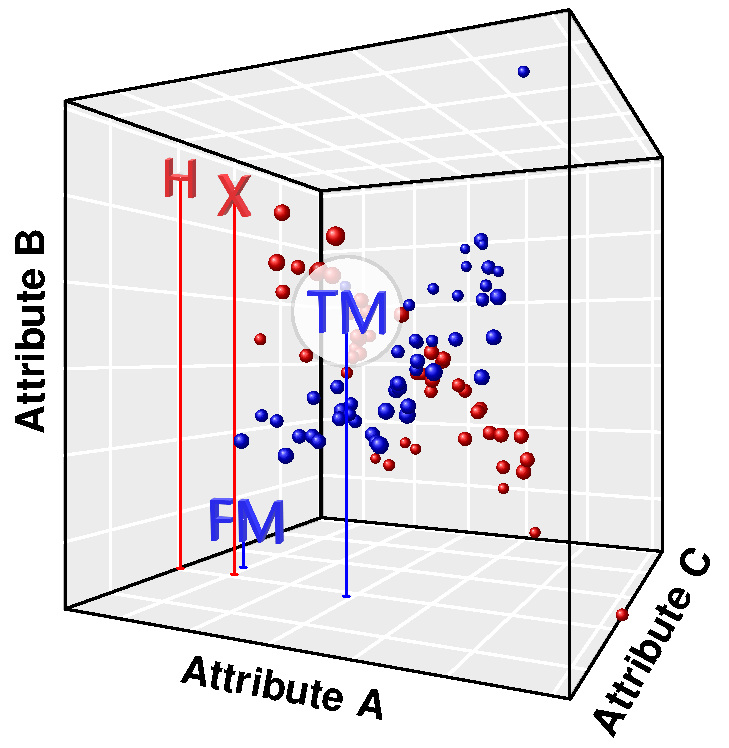
\includegraphics[width=0.8\textwidth]{nice_box_2D_points.pdf}}
%\end{minipage} \hspace{-0.4cm}
%\begin{minipage}[c]{0.5\textwidth}
%\centering
%\caption{{\bf 3D AB view}. Still working on this. }\label{fig:3d_c}
%\end{minipage}
%%\end{center}
%\end{figure}  

%\begin{figure}[ht!]
%%\begin{center}
%%\begin{minipage}[c]{0.4\textheight}
%\centering
%		\framebox{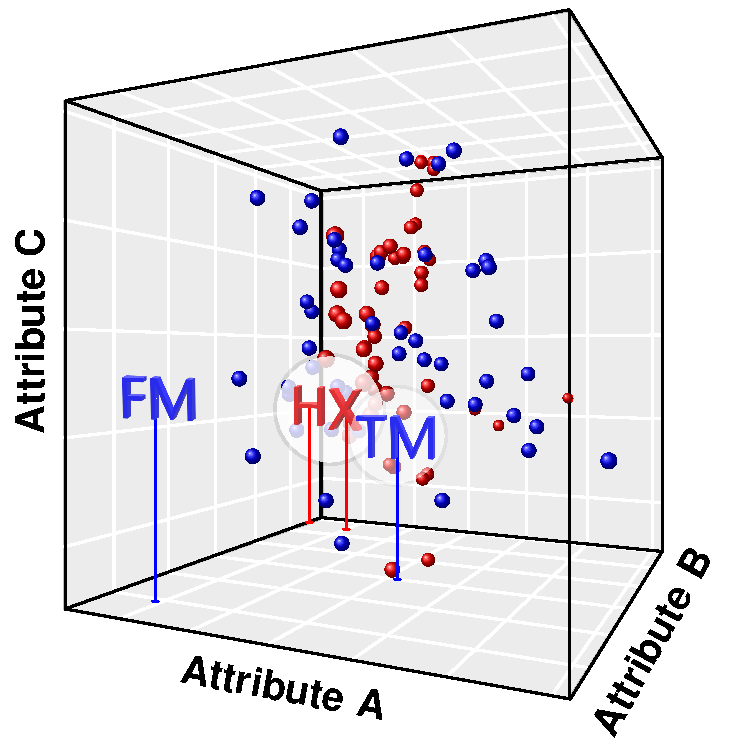
\includegraphics[width=0.8\textwidth]{nice_box_2D_points2.pdf}}
%\end{minipage} \hspace{-0.4cm}
%\begin{minipage}[c]{0.5\textwidth}
%\centering
%\caption{{\bf 3D AC view}. Still working on this. }\label{fig:3d_d}
%\end{minipage}
%%\end{center}
%\end{figure}  
Using same interaction, increase background noise genes to see degrading of A and B Relief importance because of curse of dimensionality (sparseness). 

\section{Neighborhood methods}
Nearest-neighbor projected distance (NPD) methods rely on a neighborhood algorithm for feature selection. One may specify a fixed-$k$ number of neighbors, a fixed radius, an average radius SURF, a MultiSURF radius that adapts for each instance~\cite{urbanowicz17}, or a gene-wise adaptive-$k$~\cite{mckinney13}. The definitive difference between fixed-$k$ and either fixed or adaptive radius methods is that there is always a deterministic number of neighbors in fixed-$k$ neighborhoods, but there is a variable neighborhood order in each fixed or adaptive radius method. In nearest-neighbor feature selection, neighborhood order is directly related to selected feature quality. Correlation and interaction effects change the distribution of pairwise distances between instances, which ultimately changes the probability of neighborhood inclusion for fixed or adaptive radius methods. In order to select the best set of features from data, it is important to know how pairwise feature correlation changes the optimal neighborhood order. We approach this problem by first determining the functional relationship between fixed-$k$ and MultiSURF radius in null data with no effects.

\section{Derivation of expected $k$ for multiSURF neighborhoods}
The MultiSURF radius for an instance is the mean of its distances to all other instances subtracted by $\alpha=1/2$ of the standard deviation of this mean. Previously we showed empirically for balanced case-control datasets that a good constant-$k$ approximation to the expected number of neighbors within the multiSURF radii is $k=m/6$~\cite{stir}, where $m$ is the number of samples. Here we derive a more exact theoretical mean that shows the mathematical connection between neighbor-finding methods. This fixed-$k$ approximation to MultiSURF is independent of the type of data and the particular radii of each instance in the data.
%

The distance between instances ($i,j \in \mathcal{I}$, $|\mathcal{I}|=m$) in the data set $X^{m \times p}$ of $m$ instances and $p$ attributes is calculated in the space of all attributes ($a \in \mathcal{A}$, $|\mathcal{A}|=p$) using a metric such as
\begin{equation}\label{eq:D}
% D^{(q)}_{ij}=\left(\sum_{a\in A}|\text{d}^{\text{type}}_{ij}(a)|^q\right)^{1/q},
D^{(q)}_{ij}=\left(\sum_{a\in \mathcal{A}}|\text{d}_{ij}(a)|^q\right)^{1/q},
\end{equation}
%
which is typically Manhattan ($q=1$) but may also be Euclidean ($q=2$). The quantity 
$\text{d}_{ij}(a)$,
known as a ``$\text{diff}$'' in Relief literature, is the projection of the distance between instances $i$ and $j$ onto the attribute $a$ dimension. The 
% ``type'' refers to the data type of the attribute
function $\text{d}_{ij}(a)$ supports any type of attributes
(e.g., numeric and categorical).
For example, the projected difference between two instances $i$ and $j$ for a continuous numeric ($\text{d}^{\text{num}}$) attribute $a$ may be
%\begin{equation}\label{eq:diff}
%\text{diff}^{(\text{num})}(a,(\ri,\rj))=\frac{|\text{value}(a,\ri)-\text{value}(a,\rj)%|}{\max(a)-\min(a)}.
%\end{equation}
\begin{equation}\label{eq:diff}
\begin{aligned}
\text{d}^{\text{num}}_{ij}(a)&=\text{diff}(a,(i,j))\\
                                            & = {|\hat{X}_{ia}-\hat{X}_{ja}|},
\end{aligned}
\end{equation}
where $\hat{X}$ represents the standardized data matrix $X$.
We use a simplified d$_{ij}(a)$ notation in place of the $\text{diff}(a,(i,j))$ notation that is customary in Relief-based methods.
We omit the division by $\max(a)-\min(a)$ used by Relief to constrain scores to the interval from $-1$ to $1$.
As we show in subsequent sections, NPDR scores are standardized regression coefficients with corresponding P values, so any scaling operation at this stage is unnecessary for comparing attribute scores. 
%\emph{Omit: The scaling may alleviate bias in the distance calculation. However, standardizing the data matrix $X$ ($\hat{X}$) should have the same effect without division by $\max(a)-\min(a)$, which has usual distribution properties for distances (expand).}
The numeric d$^{\text{num}}_{ij}(a)$ projection is simply the absolute difference between row elements $i$ and $j$ of the data matrix $X^{m \times p}$ for the attribute column $a$. 

We define the NPDR neighborhood set $\mathcal{N}$ of ordered pair indices as follows. Instance $i$ is a point in $p$ dimensions, and we designate the topological neighborhood of $i$ as $N_{i}$. This neighborhood is a set of other instances trained on the data $X^{m \times p}$ and depends on the type of Relief neighborhood method (e.g., fixed-$k$ or adaptive radius) and the type of metric (e.g., Manhattan or Euclidean). If instance $j$ is in the neighborhood of $i$ ($j \in N_{i}$), then the ordered pair $(i,j) \in \mathcal{N}$ for the projected-distance regression analysis. The ordered pairs constituting the neighborhood can then be represented as nested sets:
\begin{equation}\label{eq:N}
\mathcal{N}=\{\{(i, j)\}_{i=1}^{m}\}_{\{j \ne i : j \in N_{i}\}}.
\end{equation}
The cardinality of the set $\{j \ne i : j \in N_{i}\}$ is $k_i$, the number of nearest neighbors for subject $i$. 

\subsection{Predicted number of neighbors in the MultiSURF alpha neighborhood}

Regardless of the predictor data type (numeric or categorical), the distribution of the $p$ predictors (uniform, Gaussian, or binomial), or the metric used to compute distances (Manhattan or Euclidean), the $m(m-1)/2$ pairwise distances in the $p$-dimensional space are well approximated by a normal distribution. An instance $j$ is in the adaptive $\alpha$-radius neighborhood of $i$ ($j \in N^{\alpha}_{i}$) under the condition
%\begin{equation}
%\bar{D = \frac{2p}{\sqrt{\pi}}
%\end{equation}
%
%\begin{equation}
%\sigma_{D} = \frac{2p(\pi-2)}{\pi}
%\end{equation}
%
\begin{equation}
D_{ij} \le \, R_i^{\alpha} \implies j \in N^{\alpha}_{i},
\end{equation}
where the threshold radius for instance $i$ is
\begin{equation}
R_i^{\alpha} =  \bar{D}_i - \alpha \, \sigma_{\bar{D}_i}
\end{equation}
and
\begin{equation}
\bar{D}_i = \frac{1}{m-1} \sum_{j \ne i} D^{(\cdot)}_{ij}
\end{equation}
is the average of instance $i$'s pairwise distances (Eq. \ref{eq:D}) with standard deviation $\sigma_{\bar{D}_i}$. MultiSURF implements $\alpha=1/2$~\cite{urbanowicz17}.

The probability of the remaining $m-1$ instances being inside the $\alpha$-radius of instance $i$ ($R_i^{\alpha}$) can be viewed as $m-1$ Bernoulli trials each with a probability of success $q_{\alpha}$. Then the average average number of neighbors is given by
\begin{equation}
\label{eq:binomial_average}
  {\bar{k}}_{\alpha} = (m-1)q_{\alpha},
\end{equation}
from the mean of a binomial random variable. To calculate $q_{\alpha}$, we assume the distribution of distances $\{D_{ij} \}_{j \ne i}$ of neighbors of instance $i$ is normal $N(\bar{D}_i,\sigma_{\bar{D}_i})$. Our empirical studies confirm a normal distribution and that it is robust to data type and metric. Extreme violations of independence of attributes (extreme correlations or interactions) will cause the distribution to be right skewed, but this effect is difficult to observe in real data. Thus, for a Gaussian pairwise distance distribution, the probability $q_{\alpha}$ for one instance $j \ne i$ to be in the neighborhood of $i$ ($j \in N^{\alpha}_{i}$) is given by the area under the mean-centered ($\bar{D}_i$) Gaussian from $-\infty$ to $R_i^{\alpha}$. An illustration of the area computed to estimate $q_{\alpha}$ is given by Fig. \ref{fig:gaussPlot}. This integral can be written in terms of the error function (erf):
\begin{equation}
\label{eq:q_prob}
q_{\alpha} = \frac{1}{2} \left( 1 - \mathrm{erf}\left( \frac{\alpha}{\sqrt{2}} \right) \right).
\end{equation}
And finally using Eqs. (\ref{eq:binomial_average} and \ref{eq:q_prob}) we find
\begin{equation}\label{eq:kbar}
{\bar{k}}_{\alpha} = \left \lfloor \frac{m-1}{2}  \left( 1 - \mathrm{erf}\left( \frac{\alpha}{\sqrt{2}} \right) \right) \right \rfloor,
\end{equation}
where we apply the floor function to ensure the number of neighbors is integer. For data with balanced hits and misses in standard fixed-$k$ Relief, one divides this formula by 2. For multiSURF ($\alpha=1/2$), this formula gives $\bar{k}_{\alpha}^{\text{hit/miss}} = \bar{k}_{1/2}^{\text{hit/miss}} = \frac{1}{2}\bar{k}_{1/2} = .154 (m-1)$, which is very close to our previous empirical estimate $m/6$. When we compare multiSURF neighborhood methods with fixed-$k$ neighborhoods, we use $\bar{k}_{1/2}$. Using this $\alpha=1/2$ value has been shown to give good performance for simulated data sets. However, the best value for $\alpha$ is likely data-specific and may be determined through nested cross-validation and other parameter tuning methods.

\begin{figure}[ht!]
\centering
\begin{minipage}[h]{0.7\textwidth}
		\framebox{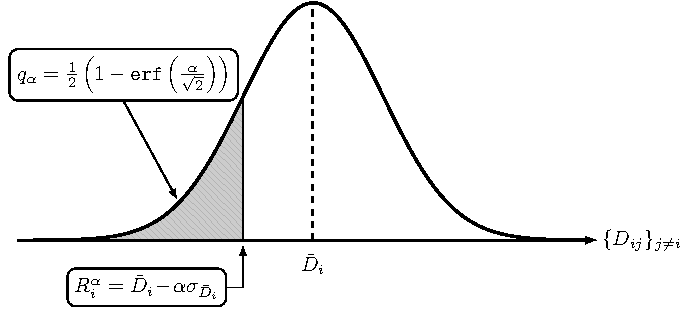
\includegraphics[width=0.95\textwidth]{shaded_bell_curve.pdf}}
\end{minipage}%\hspace{0.15cm}
\begin{minipage}[h]{0.3\textwidth}
\noindent\refstepcounter{figure}\textbf{Fig \thefigure \label{fig:gaussPlot}.} Illustration of the expected probability of a fixed instance $j$ being in the fixed radius neighborhood of another instance $i$. The fixed radius is parameterized by a fraction $\alpha$ of the standard deviation of all pairwise distances measured from instance $i$ to all possible neighbors.
\end{minipage}
\end{figure} 

\section{Optimal neighborhood parameters for detecting effects}
k or $\alpha$. 
Balancing blessing and curse of dimensionality.


\section{ICA?}

Using same interaction, increase background noise genes to see degrading of A and B Relief importance because of curse of dimensionality (sparseness).  

\section{Data simulations}

Each simulated data set $X^{(m \times p)}$ contains $m$ instances and $p$ features, where
\begin{equation}\label{eq:instance_dims}
m \in \{100, 250, 500\} \text{ and }
\end{equation}
\begin{equation}\label{eq:feature_dims}
p \in \{1000,2500,5000\}.
\end{equation}

All combinations of $m$ and $p$ were explored in order to determine how neighborhood selection parameters change with dimensionality. We considered a balanced binary outcome only so that there were exactly $m/2$ cases and $m/2$ controls. In each simulation, 10\% of the total number of features $p$ were functionally related to the outcome variable while the remaining 90\% were simply background features with no effect. Functional features were given either main or interaction effect in order to create a random mixed effects data set for which optimal neighborhood method parameters could be calculated. 

\subsection{Interaction effects}

We extend the interaction effect simulation introduced in \cite{lareau15}. This method first generates a random graph from either Erd\H{o}s-R\'{e}nyi or Scale-free degree distribution. In the control group, functional features are given large pairwise correlations with all other features. Differential correlations (interaction effects) are created by randomly permuting functional feature data entries within the case group only, which destroys and preserves the correlation in case and control groups, respectively. This method creates large effect sizes, which are easily detected by nearest-neighbor distance based methods. The reason for this ease of detection is the uniformity in low and high correlations in case and control groups, respectively. In order to establish more influence over the number of differential pairwise correlations, we simulated correlation matrices for case and control groups directly. We allowed only functional connections to be given differential correlation between case and control groups, where a functional connection is simply the presence of an edge (or link) from one feature to a functional feature in the random network that is generated.

Analogous to the interaction simulation method given in \cite{lareau15}, we give the control group high and low positive pairwise correlation between network connected and non-connected features, respectively. The average magnitudes of the high and low correlations in the control group are determined by fixed parameters $\rho^\text{hi}$ and $\rho^\text{lo}$, respectively. For all simulations, we fixed the low correlation parameter $\rho^\text{lo}$. In order to examine how interaction effect size changes with functional connection pairwise correlation, we let $\rho^\text{hi} \in \{0.2, 0.5, 0.8\}$. Interaction effect size increases and decreases monotonically as $\rho^\text{hi}$ increases and decreases, respectively. Interaction effect size is highly related to how connected a functional feature is in the random network. We control network connectivity by the probability of edge inclusion for Erd\H{o}s-R\'{e}nyi networks and fixed node degree for Scale-free networks. Similar to $\rho^\text{hi}$, interaction effect size increases and decreases monotonically as functional network connectivity increases and decreases, respectively. Furthermore, we determine interaction effect sizes by giving functional connection pairwise correlations in the case group values determined by the parameter $b^\text{int}$, which is defined as
\begin{equation}\label{eq:b_int}
b^\text{int} = - t \rho^\text{hi} + (1 - t) \rho^\text{hi}, \text{ where } t \in [0,1].
\end{equation}
As $t \to 0$, the effect size decreases monotonically. On the other hand, the effect size increases monotonically as $t \to 1$. By controlling $\rho^\text{hi}$, $b^\text{int}$, and the level of network connectivity, we have the ability to more finely control the interaction effect size than the method presented in \cite{lareau15}. 

After correlation matrices are created for cases and controls, we compute the upper triangular Cholesky factors ($U^\text{case}$ and $U^\text{ctrl}$) for each correlation matrix. We simulate null data matrices $X^\text{case}$ and $X^\text{ctrl}$ for cases and controls, respectively, such that 
\begin{equation}\label{eq:null_case_ctrl}
x^\text{case}_{ij}, x^\text{ctrl}_{ij} \sim \mathcal{N}(0,1) \quad \forall i,j.
\end{equation}
Multiplication of $X^\text{case}$ and $X^\text{ctrl}$ by the Cholesky factors $U^\text{case}$ and $U^\text{ctrl}$, respectively, produce case and control sub-matrices $Y^\text{case}$ and $Y^\text{ctrl}$ with the correlation structure described previously. These sub-matrices are then combined into a single data $m \times p$ matrix given by
\begin{equation}\label{eq:full_interaction_data}
X = \left[
\begin{array}{c}
Y^\text{ctrl} \\ [0.5ex]
\hdashline \\ [-1.7ex]
Y^\text{case}
\end{array}
\right].
\end{equation}
A diagram outlining the interaction simulation algorithm for a data set consisting of 7 features is shown in Fig.~\ref{fig:interaction_simulation_diagram}. Boxes 1 and 2 display the random network and its characteristics, such as, adjacencies and node degrees. In particular, boxes 1 and 2 show the features that are selected to be functional (highlighted in \textcolor{black!50!green}{green}). Box 3 shows the case and control correlation matrices generated using input parameters $\rho^\text{hi}$, $\rho^\text{lo}$, and $b^\text{int}$. In the control group, high correlation (\textcolor{red}{red}) is assigned to all connected pairs from the network. That is,
\begin{equation}\label{eq:control_connected_corrs}
P^\text{ctrl}_{ij} = \rho^\text{hi} + \varepsilon_{ij}, \quad \varepsilon_{ij} \sim \mathcal{N}(0,1).
\end{equation}
In both case and control groups, low correlation (\textcolor{red!45}{red}) is assigned to non-connected features from the network. These low correlations are given by
\begin{equation}\label{eq:non-connected_corrs}
P^\text{case} = P^\text{ctrl} = \rho^\text{lo} + \varepsilon_{ij}, \quad \varepsilon_{ij} \sim \mathcal{N}(0,1).
\end{equation}
In the case group, pairwise correlations associated with functional connections (\textcolor{blue!80}{blue}) from the network are assigned a correlation that is functionally related (see Eq.~\ref{eq:b_int}) to high correlations in the control group. These correlations are given by
\begin{equation}\label{eq:case_connected_corrs}
P^\text{case}_{ij} = b^\text{int} + \varepsilon_{ij}, \quad \varepsilon_{ij} \in \mathcal{N}(0,1).
\end{equation}
Other than entries associated with functional connections, the case and control correlation matrices are identical. Box 4 shows the Cholesky decompositions for $P^\text{ctrl}$ and $P^\text{case}$, which are given by
\begin{equation}\label{eq:cholesky_decomp}
\begin{aligned}
P^\text{ctrl} &= U^\text{ctrl} \left(U^\text{ctrl}\right)^\text{T} \quad \text{and}\\
P^\text{case} &= U^\text{case} \left(U^\text{case}\right)^\text{T}.
\end{aligned}
\end{equation}
Random case and control data with correlation structure determined by $P^\text{case}$ and $P^\text{ctrl}$, respectively, are created as mentioned previously (box 5). These sub-matrices are given by
\begin{equation}\label{eq:case_control_sub-mats}
\begin{aligned}
Y^\text{ctrl} &= X^\text{ctrl} \left(U^\text{ctrl}\right)^\text{T}, \quad x^\text{ctrl}_{ij} \sim \mathcal{N}(0,1) \quad \text{and}\\
Y^\text{case} &= X^\text{case} \left(U^\text{case}\right)^\text{T}, \quad x^\text{case}_{ij} \sim \mathcal{N}(0,1).
\end{aligned}
\end{equation}
The full data set, given previously by Eq.~\ref{eq:full_interaction_data}, concludes the generation of the full $m \times p$ data set $X$ with interaction effects.

\begin{figure}[H]
\centering
\begin{minipage}[h]{1\textwidth}
\framebox{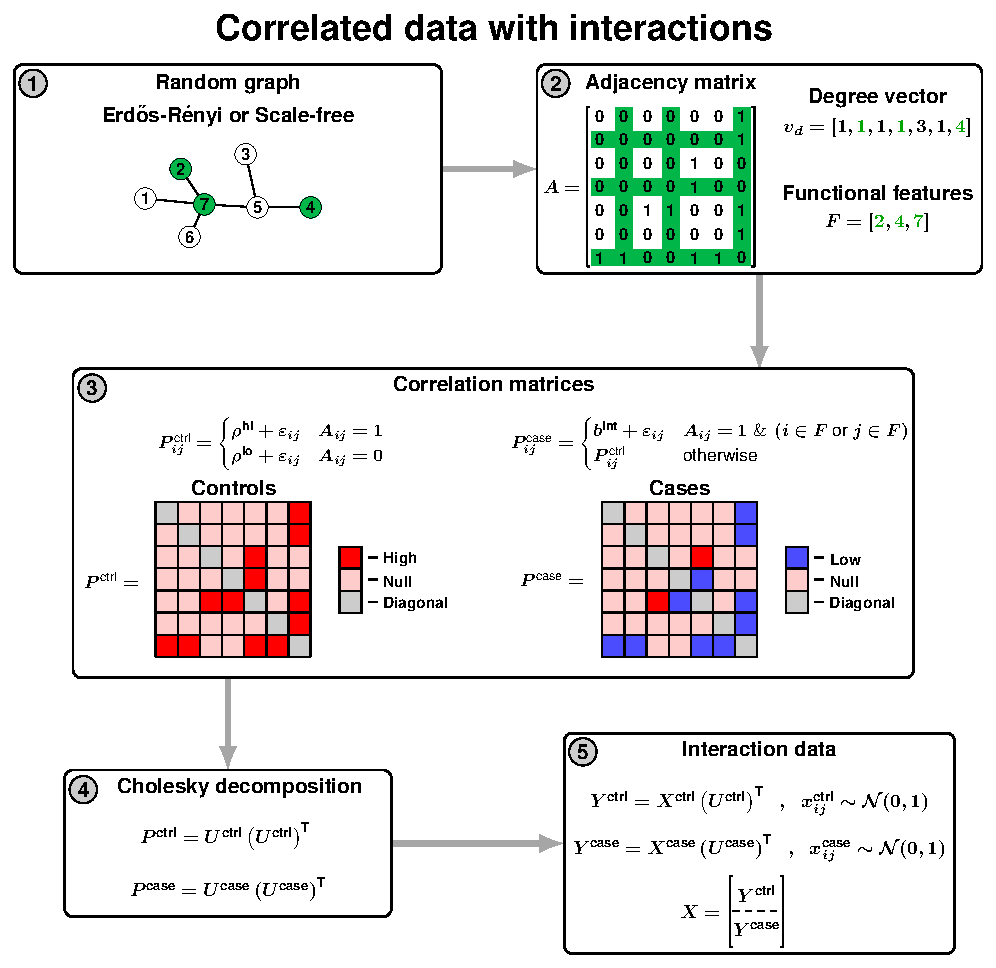
\includegraphics[width=0.98\textwidth]{interaction_simulation_method_diagram2.pdf}}
\end{minipage}

\begin{minipage}[h]{1\textwidth}
	\noindent\refstepcounter{figure}\textbf{Fig \thefigure \label{fig:interaction_simulation_diagram}.} Algorithm for interaction simulations from a random undirected network with seven nodes (or features). \textbf{Box 1:} A random network is generated, whose degree distribution is either Erd\H{o}s-R\'{e}nyi or Scale-free. \textbf{Box 2:} Adjacency matrix ($A$) and degree vector ($v_d$) corresponding to the random network are computed and functional features ($F$) are randomly selected from those with positive degree. \textbf{Box 3:} Two correlation matrices are generated for cases and controls. In the control group, high ($\rho^\text{hi}$) and low ($\rho^\text{lo}$) correlations are assigned to connected ($A_{ij}=1$) and non-connected ($A_{ij}=0$) feature pairs, respectively. In the case group, differential correlation ($b^\text{int}$) is applied to functional connections. \textbf{Box 4:} Upper triangular Cholesky factors are computed for case/control correlation matrices. \textbf{Box 5:} Standard normal random data matrices ($X^\text{ctrl}$ and $X^\text{case}$) are given correlation structure associated with case and control groups and combined into full data matrix with interaction effects ($X$).
\end{minipage}
\end{figure}

\subsection{Main effects with correlation}

\begin{figure}[H]
	\centering
	\begin{minipage}[h]{1\textwidth}
		\framebox{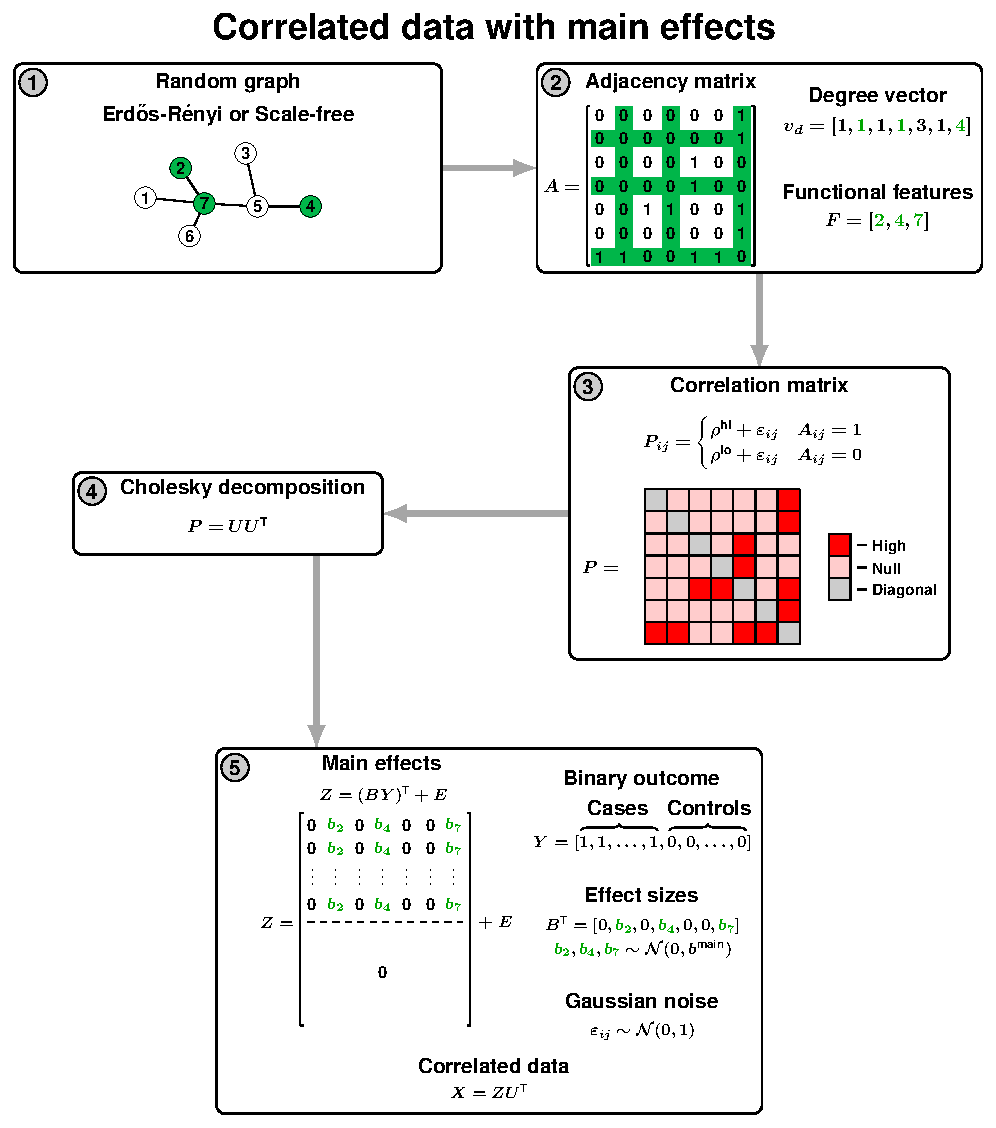
\includegraphics[width=0.98\textwidth]{main_plus_correlation_diagram.pdf}}
	\end{minipage}
	
	\begin{minipage}[h]{1\textwidth}
		\noindent\refstepcounter{figure}\textbf{Fig \thefigure \label{fig:main_plus_correlation_diagram}.} Algorithm for simulating main effects with correlation from a random undirected network with seven nodes (or features). \textbf{Box 1:} A random network is generated, whose degree distribution is either Erd\H{o}s-R\'{e}nyi or Scale-free. \textbf{Box 2:} Adjacency matrix ($A$) and degree vector ($v_d$) corresponding to the random network are computed and functional features ($F$) are randomly selected from those with positive degree. \textbf{Box 3:} Correlation matrix generated with high ($\rho^\text{hi}$) and low ($\rho^\text{lo}$) correlations assigned to connected ($A_{ij}=1$) and non-connected ($A_{ij}=0$) features, respectively. \textbf{Box 4:} Upper triangular Cholesky factors are computed for correlation matrix. \textbf{Box 5:} Main effects are simulated for functional variables ($F$) with effect sizes determined by $b^\text{main}$. Data is given correlation by multiplying main effects ($Z$) by Cholesky factor ($U$).
	\end{minipage}
\end{figure}

\bibliographystyle{unsrt}
\bibliography{BoD}   % name of bib file
\end{document}
